\documentclass[12pt,letterpaper]{article}
\usepackage[margin=1.5in]{geometry}
\usepackage[T1]{fontenc}
\usepackage[utf8]{inputenc}
\usepackage[english]{babel}
\usepackage{mathpazo}
\usepackage{microtype}
\usepackage{amsmath,amssymb,amsfonts,bm}
\usepackage{graphicx}
\usepackage{tabularx}
\usepackage{subfig}
\usepackage{booktabs}
\usepackage{xcolor}
\usepackage[colorlinks=true,linkcolor=black,citecolor=black,urlcolor=blue]{hyperref}
\usepackage{eurosym}
\newcommand{\e}{\mathrm{e}}

\title{\textbf{Incentives and Organizational Structure in Hospital Financing}}
\author{Jose Mar\'\{\i\}a Elena-Izquierdo}
\date{}

\begin{document}
\maketitle

\begin{abstract}
Efficient hospital financing depends not only on payment formulas, but also on the organizational relationships among the actors involved in care delivery. This paper studies how different organizational structures shape the optimal use of incentive payments for hospital managers and physicians under moral hazard. We develop a two-tier multi-task model and characterize the second-best solution under centralized and decentralized contracting. Numerical illustrations show how signal noise and the degree of complementarity or substitutability between tasks affect both the optimal intensity of incentives and the equilibrium effort choices of the agents.
\end{abstract}

\section*{Introduction}
Hospital care is the product of interactions among multiple agents. Payers, whether public or private, purchase services from hospitals. Hospital managers allocate human and material resources. Within the hospital, physicians, nurses, assistants, pharmacists, and other professionals perform differentiated tasks whose combined efforts determine diagnoses, treatments, and, ultimately, patient outcomes.

This multiplicity of agents and tasks has important implications for hospital financing. The first objective of this paper is therefore to model the inherently multi-agent and multi-task nature of hospital activity. A useful starting point is the literature on two-sided moral hazard in health care, where both hospitals and physicians affect performance and where contract design must account for those strategic interactions.

A second objective is to account for the institutional environment in which those contracts are implemented. In the Spanish case, public hospitals remain the dominant organizational form, but over the last decades private and not-for-profit providers, as well as public-private partnerships, have gained relevance. Beyond formal ownership, an important distinction concerns managerial autonomy. In much of the public system, regional health authorities contract services and hire personnel through relatively centralized procedures. By contrast, private and not-for-profit hospitals usually have greater discretion in staffing and in the internal design of physician compensation. In those settings, variable pay and activity-based remuneration are more common, whereas public hospitals rely more heavily on fixed salaries supplemented by relatively weak performance components.

The model developed below incorporates these alternative organizational arrangements. We analyze how incentive compatibility constraints change when the payer contracts simultaneously with the hospital and the physician, as opposed to a decentralized structure in which the payer contracts only with the hospital and the latter designs the physician's compensation. Our goal is to derive implications for the optimal intensity of incentives and for productive efficiency in a multi-task, multi-agent setting with moral hazard. The broader aim is to obtain testable implications that may later be confronted with data from the Spanish hospital system.

\section{The Model}

\subsection{Model Setup}
The model involves three agents: the purchaser of health services, who may be public or private; the hospital management board, referred to hereafter as the hospital; and the physician. The hospital and the physician jointly produce two outputs. The first is the quantity of services, interpreted for example as the number of admissions:
\begin{equation*}\label{eq:qen}
  q(a,t_1)=a+t_1+\epsilon_1
\end{equation*}
The nonnegative scalar $a$ denotes hospital effort aimed at expanding service volume, while $t_1$ is the physician's effort allocated to that same dimension. Output is affected by both efforts and by a random shock $\epsilon_1$.

The second output is intensity, used here as a proxy for quality.\footnote{Quality is difficult to define in hospital care. For tractability, the model focuses on service intensity per patient.} This dimension depends on physician effort $t_2$ and on a random shock $\epsilon_2$:
\begin{equation*}\label{eq:ien}
  i(t_2)=t_2+\epsilon_2
\end{equation*}
The hospital can influence the number of discharges but not the amount of diagnostic or therapeutic services provided per patient; that decision is assumed to rest with the physician.

The output vector is $\bm{x}=(q,i)$. The random components are $\bm{\epsilon}=(\epsilon_1,\epsilon_2)$, normally distributed with zero mean and variance-covariance matrix
\[
\Sigma=
\begin{pmatrix}
\sigma_1^2 & \sigma_{12}^2 \\
\sigma_{12}^2 & \sigma_2^2
\end{pmatrix},
\qquad
\bm{\epsilon}\sim N(\mathbf{0},\Sigma).
\]

The utilities of the three agents are:
\begin{eqnarray*}\label{utilen}
u_f &=& s(q,i)-\lambda[b(q,i)+w(q,i)]\\
u_h(b,a) &=& u_h[b(q,i)-\tau(a)+z(a)]\\
u_m(w,t_1,t_2) &=& u_m[w(q,i)-\psi(t_1,t_2)+\phi(t_1,t_2)]
\end{eqnarray*}
Here $s(q,i)$ is the payer's gross benefit from output, $b(q,i)$ is the payment to the hospital, and $w(q,i)$ is the physician's compensation. The hospital and physician incur effort costs captured by $\tau(a)$ and $\psi(t_1,t_2)$, respectively. We also allow for altruistic or vocational motives, represented by $z(a)$ for the hospital and $\phi(t_1,t_2)$ for the physician.

\subsection{First-Best Benchmark}
Under complete information, the principal observes both agents' efforts and contracts in a centralized structure.\footnote{With complete information, a decentralized structure implements the same first-best effort levels, so the centralized case is sufficient as a benchmark.} The principal solves:
\begin{eqnarray*}\label{maxf0en}
\nonumber \max\limits_{a,t_1,t_2}\,
\mathbb{E}_{\bm{\epsilon}}[u_f]
&=&
\mathbb{E}_{\bm{\epsilon}}
\left[
s(q(.),i(.))-\lambda\big(b(q(.),i(.))+w(q(.),i(.))\big)
\right]\\
\nonumber \text{subject to }\\
\mathbb{E}_{\bm{\epsilon}}[u_h] &\geq& u_h(\bar{b})\\
\mathbb{E}_{\bm{\epsilon}}[u_m] &\geq& u_m(\bar{w})
\end{eqnarray*}
where $u_h(\bar{b})$ and $u_m(\bar{w})$ are the reservation utilities of the hospital and the physician.

Given a realization of $\bm{\epsilon}$, the first-order conditions are:
\begin{eqnarray*}
  s_q &=& \lambda b_q-\mu_1[u_h'(b_q-\tau_a+z_a)]\\
  s_q &=& \lambda w_q-\mu_2[u_m'(w_q-\psi_{t_1}+\phi_{t_1})]\\
  s_i &=& \lambda w_i-\mu_2[u_m'(w_i-\psi_{t_2}+\phi_{t_2})]
\end{eqnarray*}
The principal can then implement the optimal effort vector $(a^*,t_1^*,t_2^*)$ and make both participation constraints bind with lump-sum transfers:
\begin{eqnarray*}
b(q)=H &=& \bar{b}+\tau(a^*)-z(a^*)\\
w(q,i)=M &=& \bar{w}+\psi(t_1^*,t_2^*)-\phi(t_1^*,t_2^*)
\end{eqnarray*}
such that
\begin{eqnarray*}
\mathbb{E}_{\bm{\epsilon}}[u_h(H;a^*)] &=& u_h(\bar{b})\\
\mathbb{E}_{\bm{\epsilon}}[u_m(M;t_1^*,t_2^*)] &=& u_m(\bar{w})
\end{eqnarray*}

The principal's problem becomes:
\begin{eqnarray*}\label{maxf05en}
\nonumber \max\limits_{a,t_1,t_2}\,
\mathbb{E}_{\bm{\epsilon}}[u_f]
&=&
\mathbb{E}_{\bm{\epsilon}}
\left[
s(q(.),i(.))-\lambda\big(\bar{b}+\tau(a)-z(a)+\bar{w}+\psi(t_1,t_2)-\phi(t_1,t_2)\big)
\right]
\end{eqnarray*}

The first-order conditions are:
\begin{eqnarray}
  s_q+\lambda z_a &=& \lambda\tau_a \\
  s_q+\lambda\phi_{t_1} &=& \lambda\psi_{t_1} \\
  s_i+\lambda\phi_{t_2} &=& \lambda\psi_{t_2}
\end{eqnarray}
Combining them yields:
\begin{equation}\label{cpo1en}
    \tau_a-z_a=\psi_{t_1}-\phi_{t_1}
\end{equation}
and
\begin{equation}\label{cpo2en}
\frac{s_q}{s_i}=
\frac{\psi_{t_1}-\phi_{t_1}}{\psi_{t_2}-\phi_{t_2}}=
\frac{\tau_a-z_a}{\psi_{t_2}-\phi_{t_2}}
\end{equation}

Equation \ref{cpo1en} states that the marginal net cost of producing quantity must be equalized across the hospital and the physician. Equation \ref{cpo2en} requires the payer's marginal rate of substitution between quantity and intensity to equal the marginal rate of transformation in production. The first-best levels of physician effort on both tasks can therefore be determined jointly, while hospital effort follows from the equalization condition. One implication is that, if a public or not-for-profit hospital has a stronger altruistic component than a for-profit hospital, the principal can induce a higher effective effort level with a lower explicit compensation requirement.

\section{Contracting Under Moral Hazard}
We now move to the more realistic case in which the principal cannot observe effort directly and must rely on output as a noisy signal. The problem becomes one of balancing productive efficiency against risk sharing. Following the standard Holmstrom-Milgrom framework, we assume exponential utility for the agents, risk neutrality for the principal, and linear compensation schemes.

\subsection{Centralized Structure}
The hospital and physician utilities are:
\begin{eqnarray*}
  u_h(b,a) &=& -\e^{-\rho[b(q,i)-\tau(a)+z(a)]} \\
  u_m(w,t_1,t_2) &=& -\e^{-\eta[w(q,i)-\psi(t_1,t_2)+\phi(t_1,t_2)]}
\end{eqnarray*}
where $\rho$ and $\eta$ are the coefficients of absolute risk aversion for the hospital and the physician, respectively.

Effort costs take the form:
\begin{eqnarray*}
  \tau(a) &=& \frac{1}{2}\tau a^2, \qquad \tau>0\\
  \psi(t_1,t_2) &=& \frac{1}{2}(\psi_1t_1^2+\psi_2t_2^2)+\psi_{12}t_1t_2,\\
&& \qquad \text{where } \psi_1>0,\ \psi_2>0,\ \psi_{12}^2\in[0,\psi_1\psi_2]
\end{eqnarray*}
The parameter $\psi_{12}$ measures the degree of complementarity or substitutability between the physician's two tasks. Altruistic motives are assumed to be linear:
\begin{eqnarray*}
  z(a) &=& z_1a,\qquad z_1\geq 0\\
  \phi(t_1,t_2) &=& \phi_1t_1+\phi_2t_2,\qquad \phi_1,\phi_2\geq 0
\end{eqnarray*}

Because effort is not observable, the principal uses linear compensation rules based on realized outputs:
\begin{eqnarray*}
  b(q) &=& f+bq \\
  w(q,i) &=& F+Bq+Di
\end{eqnarray*}
where $f$ and $F$ are fixed components and $b$, $B$, and $D$ are the variable incentive parameters attached to quantity and intensity.

The timing of the centralized problem is illustrated in Figure \ref{fig1en}.
\begin{figure}[htbp!]
  \centering
  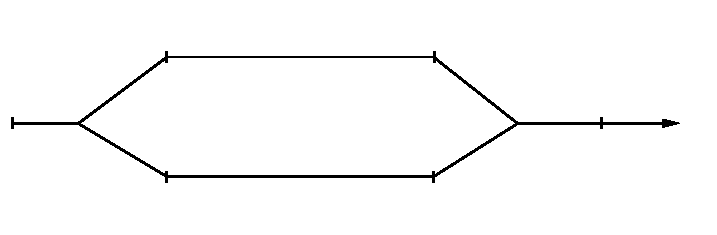
\includegraphics[width=16cm]{fig00c.pdf}
  \caption{Timeline in a centralized structure}\label{fig1en}
\end{figure}

Using the first-order approach and certainty equivalents, the incentive coefficients imply:
\begin{eqnarray*}
b^C&=&\tau a-z_1\\
B^C&=&\psi_1t_1+\psi_{12}\bar{t}_2-\phi_1\\
D^C&=&\psi_2t_2+\psi_{12}\bar{t}_1-\phi_2
\end{eqnarray*}
and the second-best effort levels are:
\begin{eqnarray}
a^{C}&=&\frac{b+z_1}{\tau}\label{asoen}\\
t_1^{C}&=&\frac{(B+\phi_1)\psi_2-(D+\phi_2)\psi_{12}}{\psi_1\psi_2-\psi_{12}^2}\label{t1soen}\\
t_2^{C}&=&\frac{(D+\phi_2)\psi_1-(B+\phi_1)\psi_{12}}{\psi_1\psi_2-\psi_{12}^2}\label{t2soen}
\end{eqnarray}

Assuming independent shocks ($\sigma_{12}=0$), the optimal incentive powers are:
\begin{eqnarray}
b^C&=&\frac{1}{\lambda(1+\rho\sigma_1^2\tau)}\label{bsoen}\\
B^C&=&\frac{\psi_2-\psi_{12}(1-\lambda D^C)}{\lambda[\psi_2+\eta\sigma_1^2(\psi_1\psi_2-\psi_{12}^2)]}\label{Bso1en}\\
D^C&=&\frac{\psi_1-\psi_{12}(1-\lambda B^C)}{\lambda[\psi_1+\eta\sigma_2^2(\psi_1\psi_2-\psi_{12}^2)]}\label{Dso1en}
\end{eqnarray}
Solving jointly for $B^C$ and $D^C$ gives:
\begin{eqnarray}
B^C&=&\frac{1+\eta\sigma_2^2(\psi_2-\psi_{12})}{\lambda[1+\sigma_1^2\sigma_2^2\eta^2(\psi_1\psi_2-\psi_{12}^2)+\eta(\sigma_1^2\psi_1+\sigma_2^2\psi_2)]}\label{Bso2en}\\
D^C&=&\frac{1+\eta\sigma_1^2(\psi_1-\psi_{12})}{\lambda[1+\sigma_1^2\sigma_2^2\eta^2(\psi_1\psi_2-\psi_{12}^2)+\eta(\sigma_1^2\psi_1+\sigma_2^2\psi_2)]}\label{Dso2en}
\end{eqnarray}

Several implications follow from the centralized solution:
\begin{itemize}
\item In contrast with the first-best benchmark, the second-best contract does not depend on the altruistic component of either agent.
\item When the physician's tasks are substitutes ($\psi_{12}>0$), the optimal incentive powers on quantity and intensity move together.
\item Incentives are independent across agents: changing the hospital incentive parameter does not affect the physician's optimal incentive coefficients.
\item When intensity is very noisy and tasks are close substitutes, the optimal contract tends toward weak or null incentives for the physician and places more of the variable compensation on the hospital.
\end{itemize}

\subsection{Decentralized Structure}
Under decentralization, the payer contracts only with the hospital, and the hospital in turn designs the physician's contract. Moral hazard therefore applies both to the payer-hospital relation and to the hospital-physician relation. Solving the game by backward induction, we first characterize the hospital's problem and then derive the payer's optimal contract. The sequence of decisions is shown in Figure \ref{fig2en}.

\begin{figure}[htbp!]
  \centering
  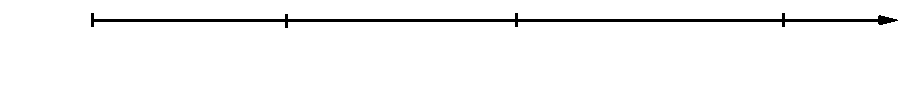
\includegraphics[width=15cm]{fig00d.pdf}
  \caption{Timeline in a decentralized structure}\label{fig2en}
\end{figure}

Using the corresponding certainty equivalents, the hospital solves:
\begin{eqnarray*}
\max\limits_{a,B,D}\ \mathbb{E}_{\bm{\epsilon}}[u_h]
&=&
f+(b-B)(a+t_1)+(d-D)t_2+z_1a-M\\
\nonumber \text{subject to }&&\\
t_1=t_1^{D}&=&\frac{(B+\phi_1)\psi_2-(D+\phi_2)\psi_{12}}{\psi_1\psi_2-\psi_{12}^2}\\
t_2=t_2^{D}&=&\frac{(D+\phi_2)\psi_1-(B+\phi_1)}{\psi_1\psi_2-\psi_{12}^2}\\
\hat{w}&=&\bar{w}
\end{eqnarray*}
where $M$ collects effort costs, the physician's risk premium, and the fixed component of the physician's compensation.

Let $\theta=(\rho+\eta)$ and $\delta=\psi_1\psi_2-\psi_{12}^2$. The optimal variable payments to the physician are:
\begin{eqnarray*}
B^D&=&\frac{b(1+\sigma_1^2\rho\psi_1+\sigma_2^2\theta(\rho\delta\sigma_1^2+\psi_2))-d\eta\sigma_2^2\psi_{12}}{1+\psi_1\theta\sigma_1^2+\theta\sigma_2^2(\theta\delta\sigma_1^2+\psi_2)}\\
D^D&=&\frac{d(1+\sigma_2^2\rho\psi_2+\sigma_1^2\theta(\rho\delta\sigma_2^2+\psi_1))-b\eta\sigma_2^2\psi_{12}}{1+\psi_2\theta\sigma_2^2+\theta\sigma_1^2(\theta\delta\sigma_2^2+\psi_1)}
\end{eqnarray*}
These expressions determine the physician's equilibrium efforts $t_1(b,d)$ and $t_2(b,d)$ as functions of the hospital's own incentive parameters.

The payer's problem is then:
\begin{eqnarray*}
\max\limits_{q,i,b,d}\ \mathbb{E}_{\bm{\epsilon}}[u_f]
&=&
a+t_1+t_2-\lambda\big(f+b(a+t_1)+dt_2\big)\\
a^D&=&\frac{b+z_1}{\tau}\\
t_1^D&=&t_1(b,d)\\
t_2^D&=&t_2(b,d)\\
\hat{b}&=&\bar{b}
\end{eqnarray*}

The general solution is algebraically cumbersome. For the tractable case in which tasks are independent in the physician's cost function ($\psi_{12}=0$), closed-form expressions can be derived for the relevant incentive parameters and effort levels. The key qualitative results are more important than the formulas themselves. As in the centralized case, altruistic parameters do not appear in the optimal variable components. However, unlike the centralized case, incentives are interconnected across hierarchical levels by construction.

Comparing the decentralized and centralized structures in the independent-task case shows that hospital effort on quantity is higher under decentralization, whereas physician effort on intensity is lower. Whether physician effort on quantity is higher under centralization or decentralization depends on the relative marginal costs of quantity production and on the agents' risk-aversion parameters. More generally, once the hospital internalizes the downstream contracting problem, organizational structure becomes an essential determinant of the final allocation of effort.

\section{Comparing Organizational Structures}
The decentralized solution is sufficiently complex that clean comparative statics are difficult to derive for the general case. For that reason, it is useful to complement the analytical results with numerical illustrations. We focus on two questions: how the interaction between the physician's tasks affects incentives and effort, and how changes in the noisiness of the output measures modify those results.

\subsection{Changes in Task Interaction}
Figure \ref{fig3en} plots optimal incentive powers over a grid of values for $\psi_{12}$, ranging from strong complementarity to strong substitution.
\begin{figure}[htbp!]
  \centering
  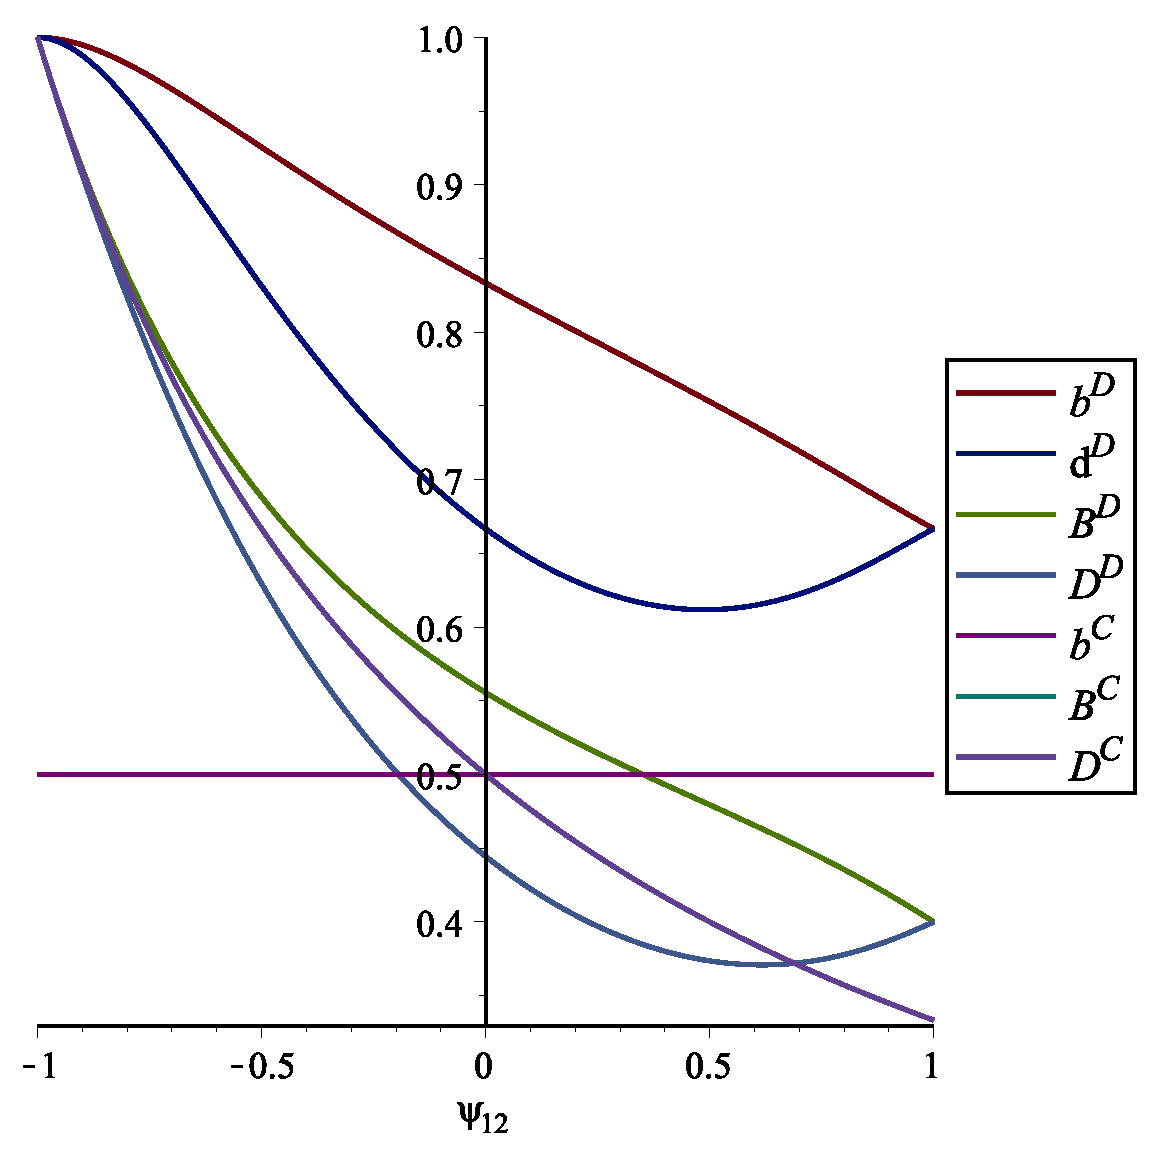
\includegraphics[width=8cm]{gr1-eps-converted-to.pdf}
  \caption{Optimal incentives under decentralized (D) and centralized (C) structures}\label{fig3en}
\end{figure}

Except for the constant hospital incentive on quantity under centralized contracting, all variable payments respond to the interaction between the physician's tasks. When tasks are strong complements, incentive powers are high and tend to converge across contracts. As substitutability increases, incentives tied to quantity tend to fall, while those linked to intensity may rise beyond a threshold. A particularly interesting result appears when tasks become nearly perfect substitutes: under centralized contracting, incentives for the physician collapse toward zero, whereas under decentralization the payer still relies on relatively strong incentives transmitted through the hospital's internal contract.

Figure \ref{fig4en} translates those incentive patterns into effort differences between organizational structures.
\begin{figure}[htbp!]
  \centering
  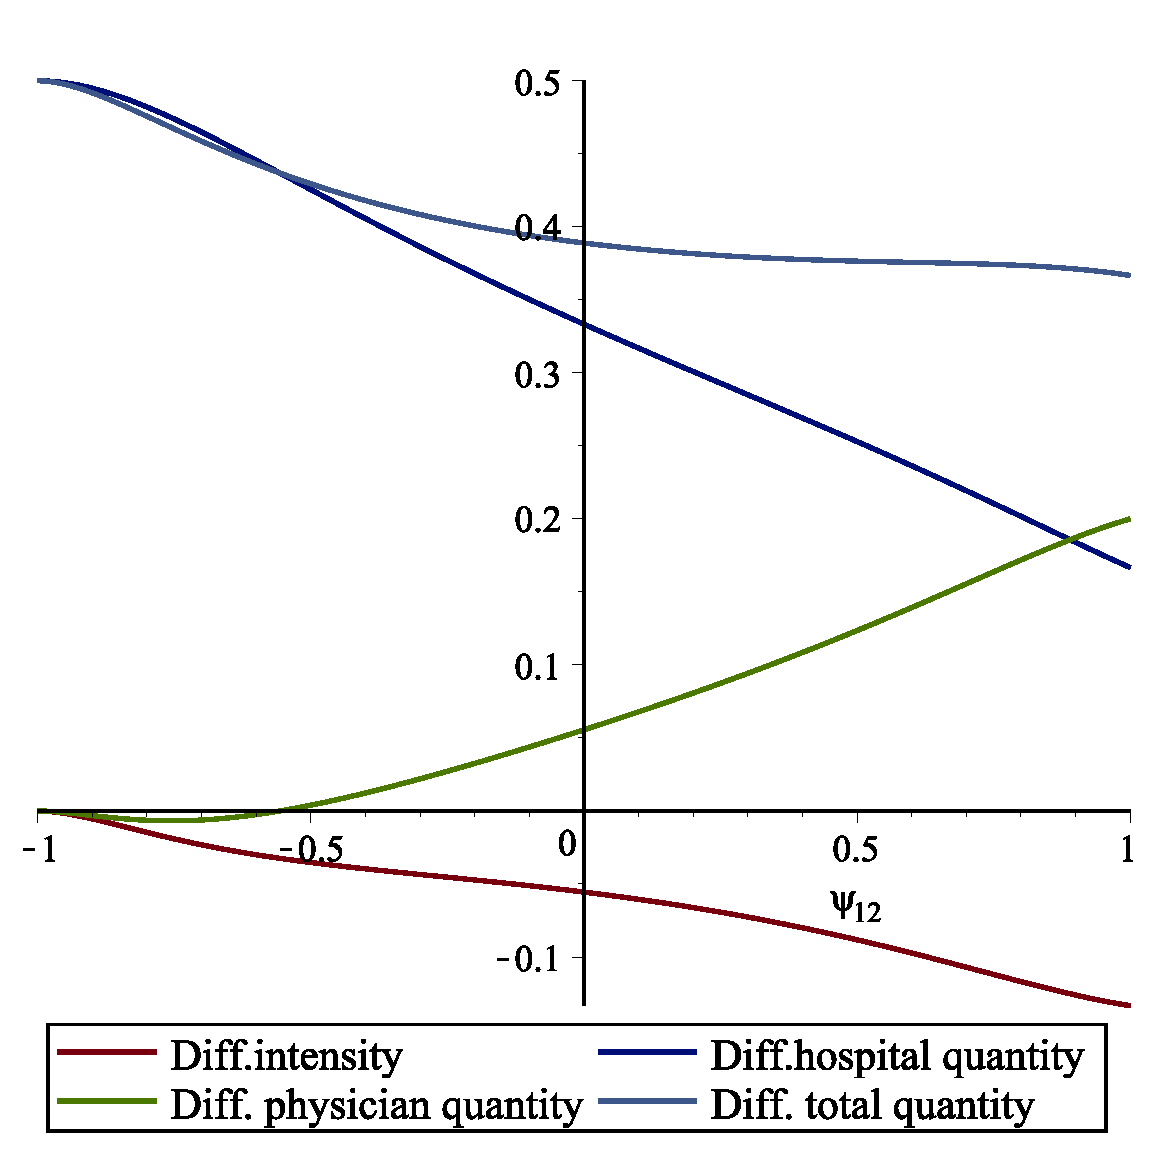
\includegraphics[width=8cm]{gr2-eps-converted-to.pdf}
  \caption{Effort differences: decentralized minus centralized}\label{fig4en}
\end{figure}

Total effort on quantity is generally higher when the principal contracts only with the hospital. As substitutability increases, decentralization shifts incentives toward quantity production, while centralization preserves relatively stronger incentives for intensity. When quantity is measured perfectly ($\sigma_1=0$), the two structures deliver the same total quantity and achieve the first-best allocation in that dimension, though intensity remains lower under decentralization. When intensity is measured without noise ($\sigma_2=0$), both structures attain the first-best level of intensity, while quantity remains higher under decentralization.

\begin{figure}[htbp!]
  \centering
  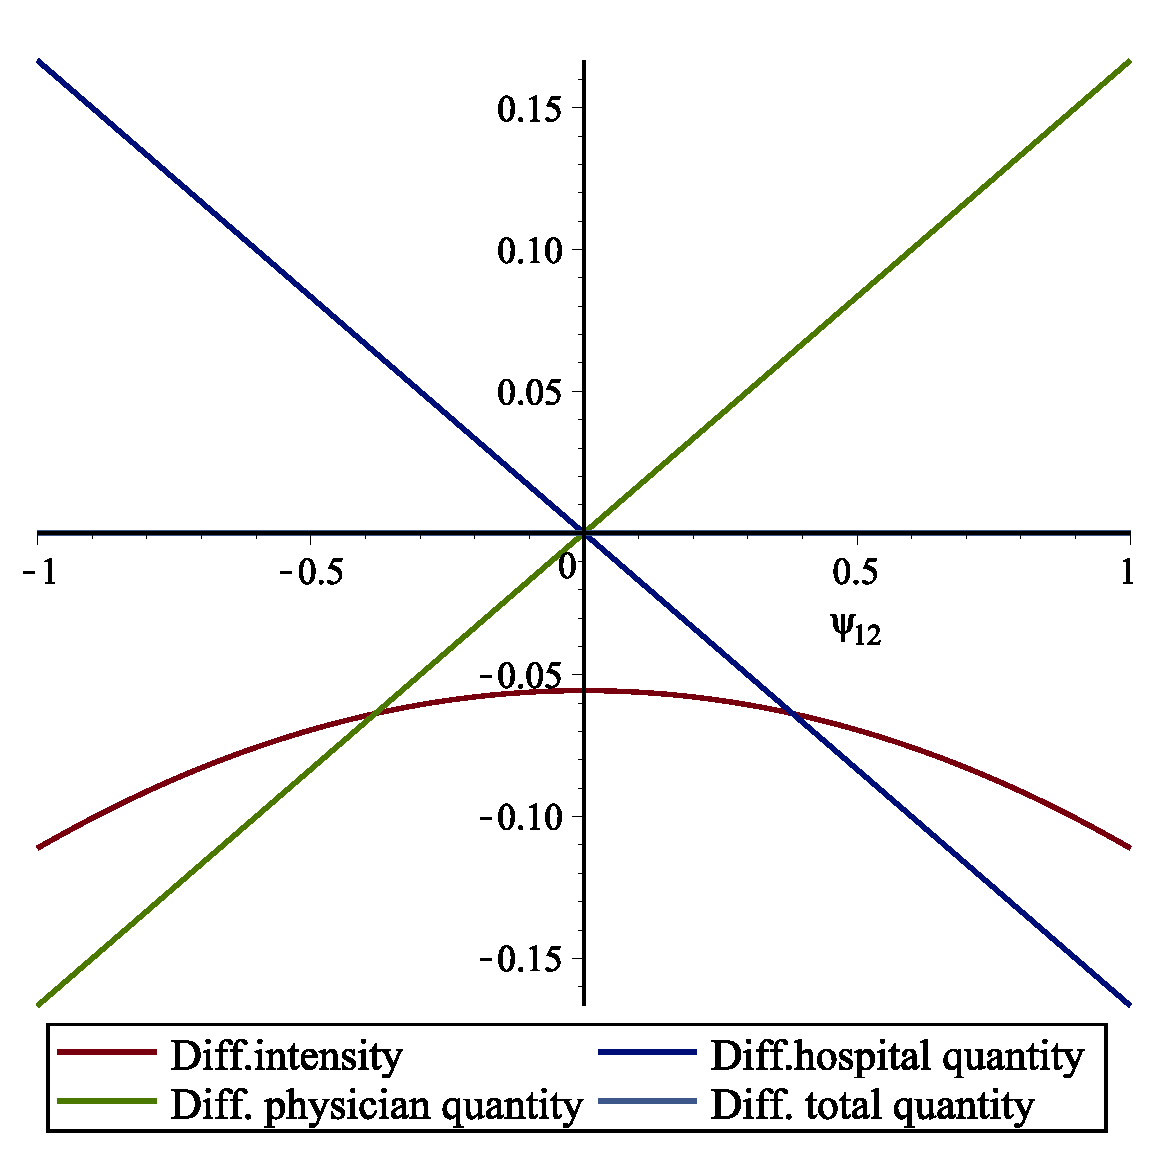
\includegraphics[width=8cm]{gr3-eps-converted-to.pdf}
  \caption{Effort differences when $\sigma_1=0$}\label{fig5en}
\end{figure}

\begin{figure}[htbp!]
  \centering
  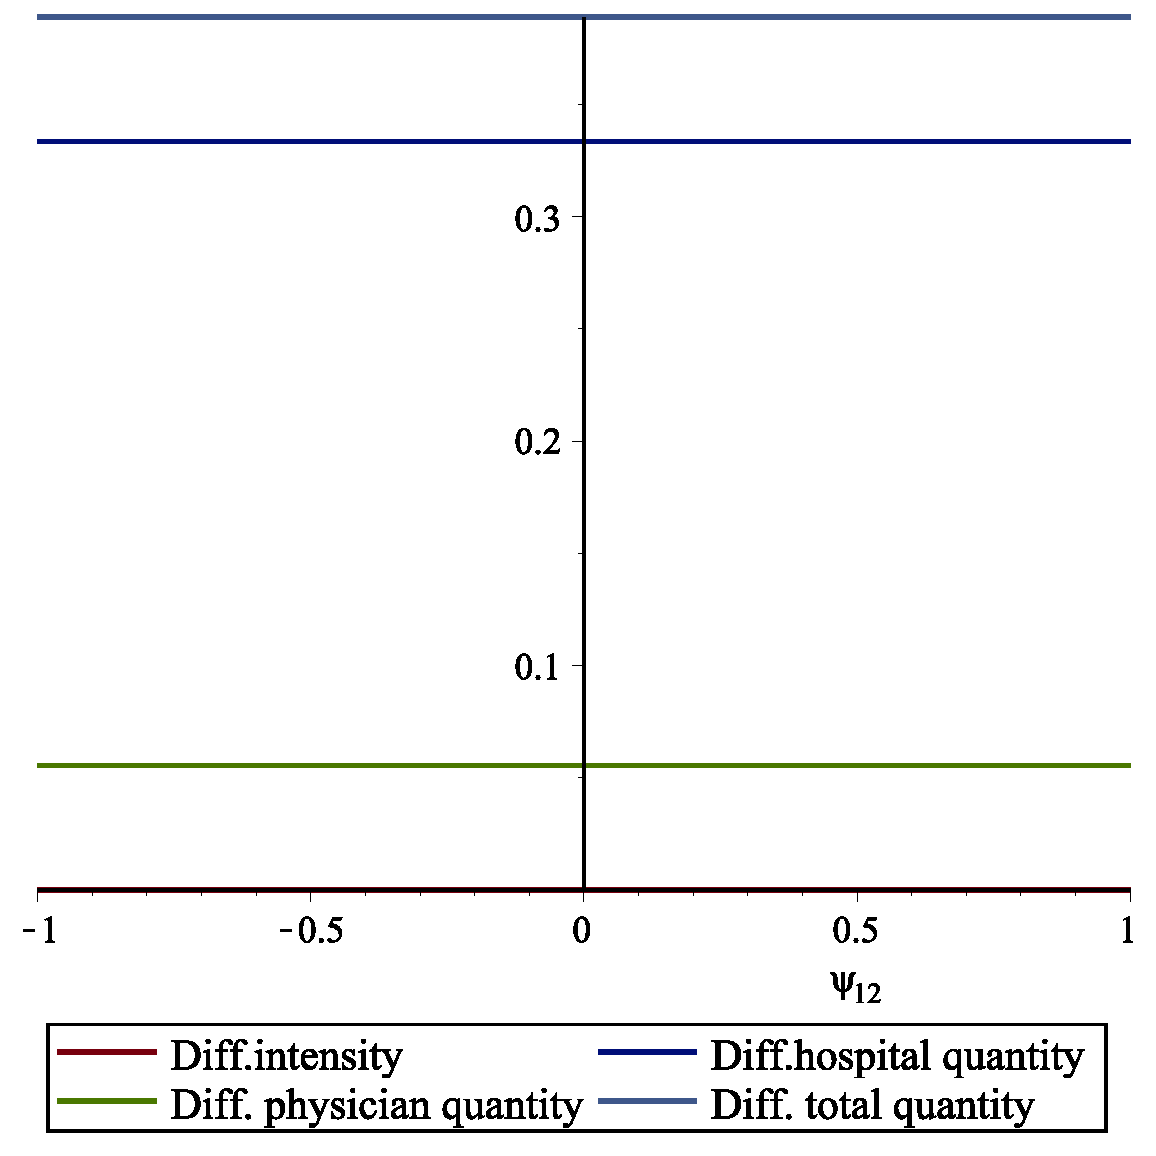
\includegraphics[width=8cm]{gr4-eps-converted-to.pdf}
  \caption{Effort differences when $\sigma_2=0$}\label{fig6en}
\end{figure}

\subsection{Imprecise Measurement of Outcomes}
We now examine how optimal incentives and effort levels react when output measures become noisier for a fixed value of $\psi_{12}$. Figure \ref{fig7en} shows the effect of increasing $\sigma_1$ when tasks are imperfect substitutes ($\psi_{12}=0.5$).
\begin{figure}[htbp!]
  \centering
  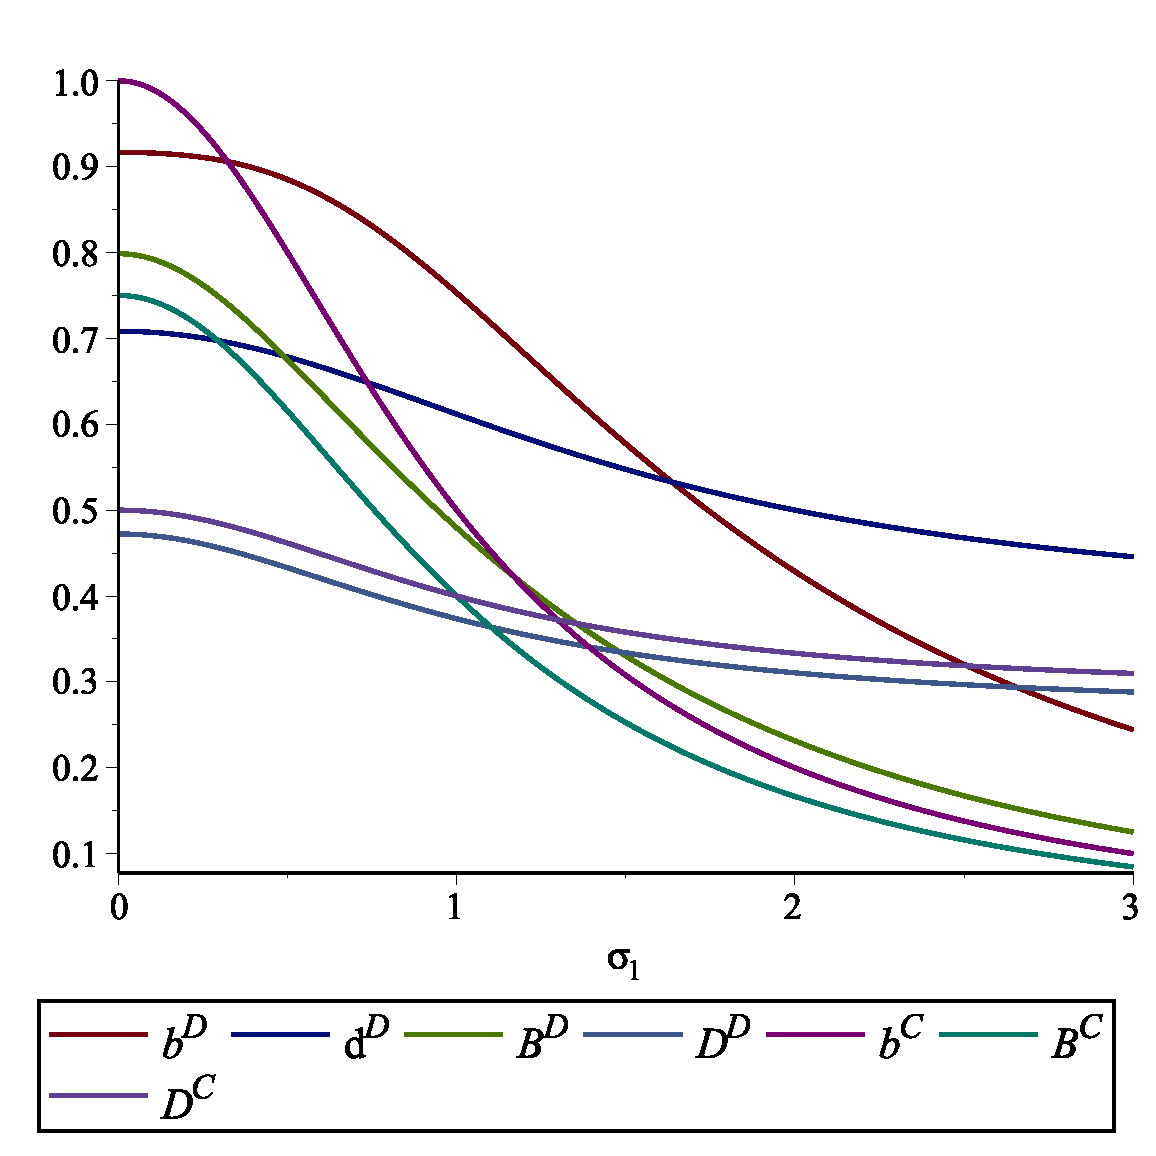
\includegraphics[width=8cm]{gr5-eps-converted-to.pdf}
  \caption{Optimal incentives as $\sigma_1$ increases}\label{fig7en}
\end{figure}

All incentive parameters decline as quantity becomes noisier. Incentives tied to quantity tend to zero, while those tied to intensity converge to positive asymptotic values. The associated effort differentials are displayed in Figure \ref{fig8en}.
\begin{figure}[htbp!]
  \centering
  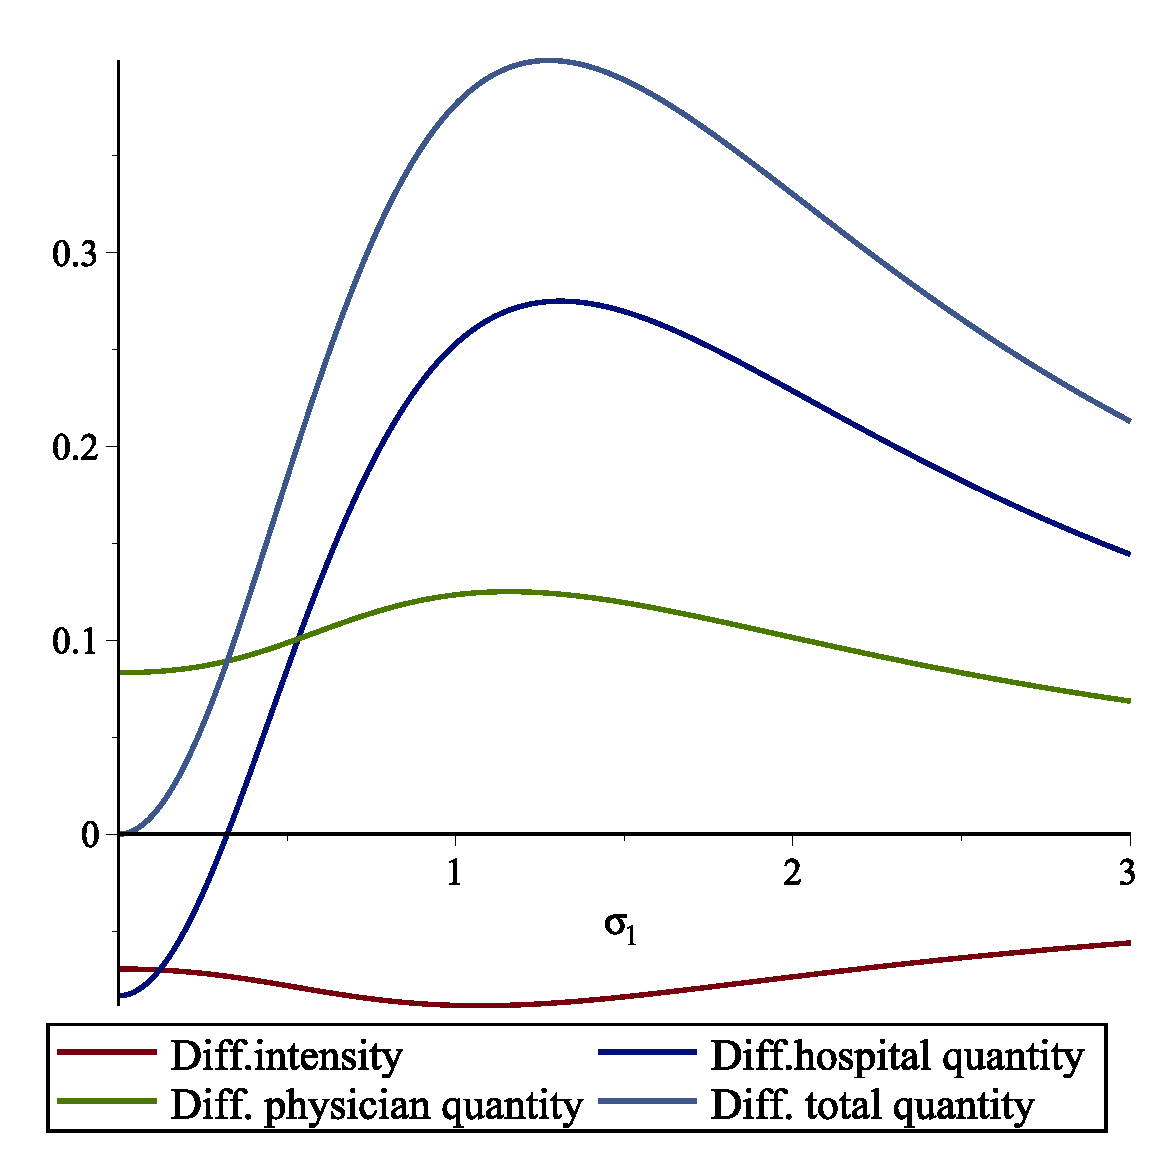
\includegraphics[width=8cm]{gr6-eps-converted-to.pdf}
  \caption{Effort differences as $\sigma_1$ increases}\label{fig8en}
\end{figure}

Intensity remains higher under centralization, whereas total quantity remains higher under decentralization. In the limit, hospital effort on quantity converges across structures, but physician effort on quantity remains higher under decentralization.

We can perform the symmetric exercise for the variance of the intensity signal. Figure \ref{fig9en} shows that, as $\sigma_2$ increases, all incentives tied to intensity decrease toward zero. Quantity incentives also fall, except for the hospital's centralized quantity incentive, which is independent of $\sigma_2$.
\begin{figure}[htbp!]
  \centering
  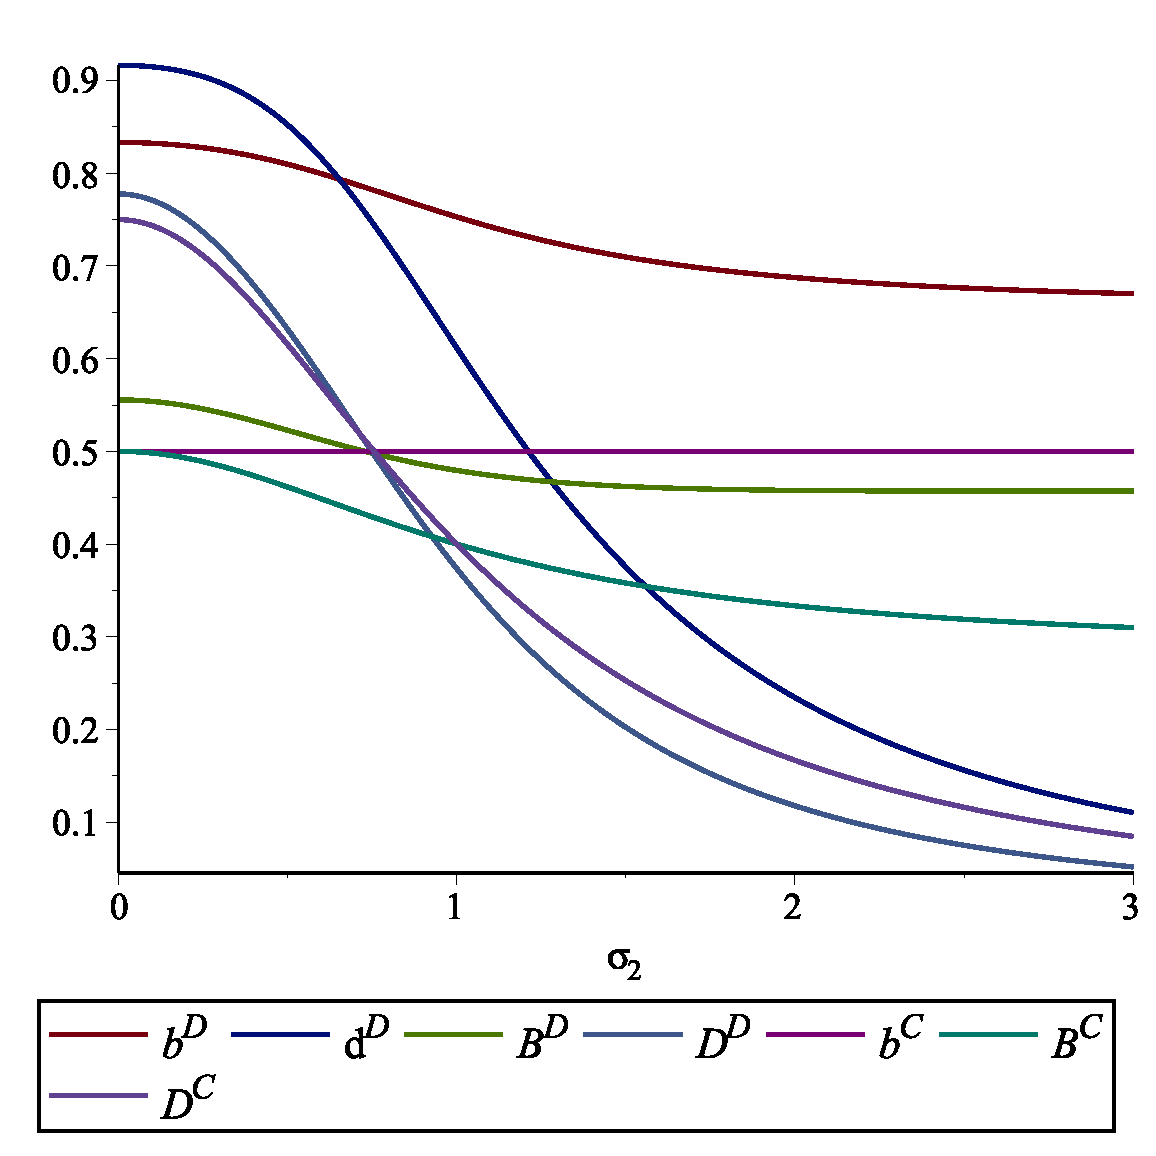
\includegraphics[width=8cm]{gr7-eps-converted-to.pdf}
  \caption{Optimal incentives as $\sigma_2$ increases}\label{fig9en}
\end{figure}

The induced effort differences are summarized in Figures \ref{fig10en} and \ref{fig11en}.
\begin{figure}[htbp!]
  \centering
  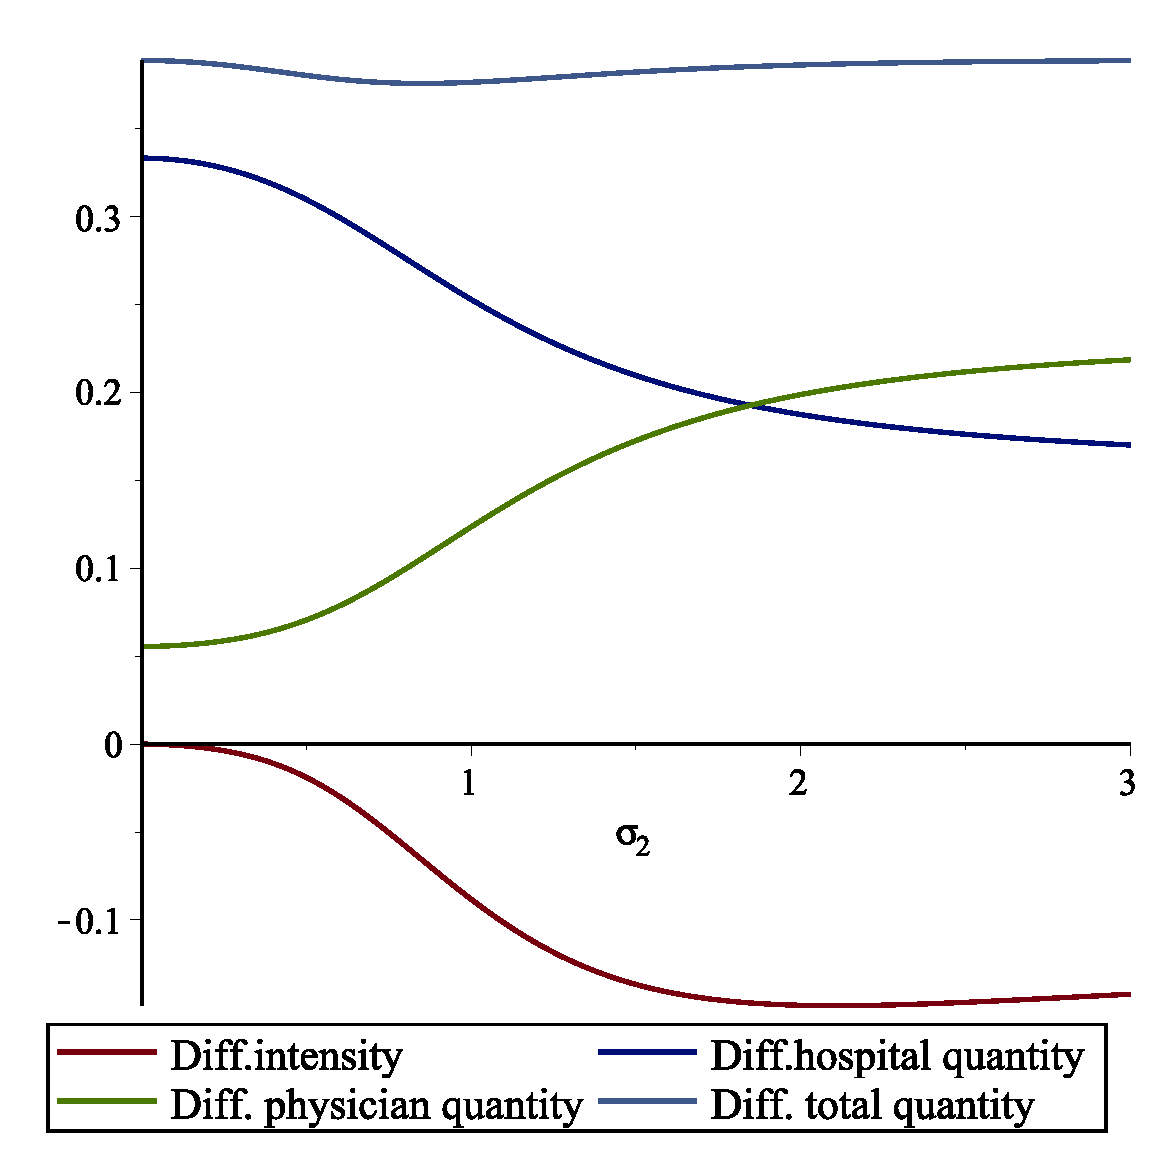
\includegraphics[width=8cm]{gr8-eps-converted-to.pdf}
  \caption{Effort differences as $\sigma_2$ increases with imperfect substitutes ($\psi_{12}=0.5$)}\label{fig10en}
\end{figure}

\begin{figure}[htbp!]
  \centering
  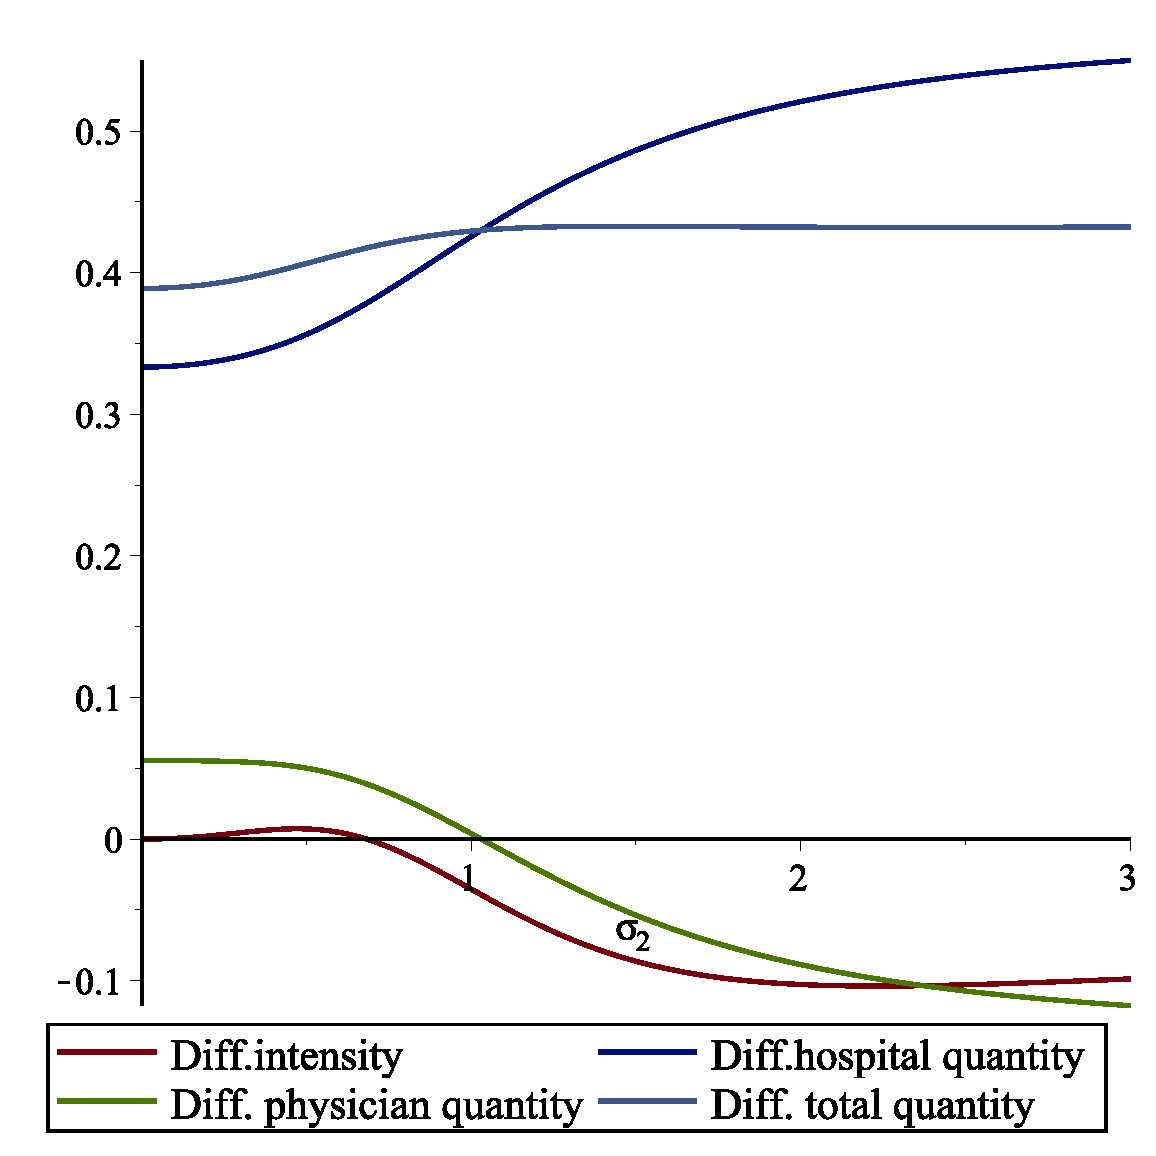
\includegraphics[width=8cm]{gr9-eps-converted-to.pdf}
  \caption{Effort differences as $\sigma_2$ increases with imperfect complements ($\psi_{12}=-0.5$)}\label{fig11en}
\end{figure}

With imperfect substitution, quantity remains higher under decentralization while intensity remains higher under centralization. With complementary tasks, the pattern is more nuanced: for low values of $\sigma_2$, decentralization may dominate in quantity and even in intensity, but as noise rises the centralized structure increasingly dominates physician performance.

\section{Conclusions}
This paper develops a model of hospital financing with multiple agents, multiple outputs, and moral hazard. The framework highlights that the effectiveness of incentive schemes depends not only on information problems, but also on the organizational architecture through which contracts are implemented.

In the full-information benchmark, the principal uses lump-sum transfers, leaves agents at their reservation utilities, and chooses efforts to equalize relevant marginal conditions across tasks and agents. Under asymmetric information, by contrast, linear incentive contracts emerge from the trade-off between insurance and effort provision.

The comparison between centralized and decentralized contracting yields three broad conclusions. First, altruistic or vocational motives affect effort choices in the first-best benchmark, but they do not alter the optimal variable components of the second-best contracts. Second, organizational structure matters because it changes how incentive problems are internalized: incentives are independent across agents under centralized contracting, whereas they become strategically linked under decentralization. Third, the relative performance of each structure depends on both technological interaction between tasks and measurement noise. In general, centralized structures tend to perform better in the intensity dimension, while decentralized structures tend to induce greater total quantity.

The simulations reinforce this point. When physician tasks are close substitutes, centralized contracting tends to weaken or eliminate physician incentives, while decentralized contracting preserves stronger powered incentives through the hospital. When output measures become noisier, the corresponding incentive powers fall, but the organizational structure continues to shape the direction of effort reallocation. The source of informational friction therefore does not map mechanically into a single preferred organizational design.

These theoretical results suggest several empirical applications. One possibility is to compare efficiency outcomes across public, not-for-profit, and for-profit hospitals under different payment mechanisms and organizational arrangements. Another is to estimate how low-powered and high-powered incentives interact with hospital autonomy in panel data for the Spanish hospital system.

\end{document}

